\section{Design and Implementation}

Although some projects build entire or partially custom blockchain network software, using a framework like Hyperledger Composer is a much more streamlined way to get a fast functioning prototype.

The baseline for the design will be the written list of requirements, mainly the functional requirements part, and the specifications of the Hyperledger projects.

The design can be divided into 4 parts:
\begin{itemize}
    \item Model Design for a Composer Business Network
    \item Access Control Design and Identity Management
    \item Network Topology and Deployment
    \item Integrating Existing Systems and Building External Applications
\end{itemize}

These parts are not necessarily sequential, but following the listed order may bring about the best results in development. Since time was an issue and the dissertation already included aspects other than the development, the scope of the development itself could not be broad enough to include a deep exploration of all the aspects listed.

Therefore, the project here presented focuses more on the quality and functional aspects of applying blockchain to the supply chain, and not so much on the quantitative part, which would include tests to the efficiency of the network (throughput, latency). What this means is that the development had a bigger focus on the model design, access control design,identity management and the implementation and validation of these aspects than on building and testing a realistic node topology. The scope for the last item, integrating existing systems and building external applications,was also narrowed down to the essential.

This section is divided in several parts to explain in which way these items were approached, so that conclusions can then be taken to reach an answer to the question: \textbf{"Is it possible to build a feasible architectural design, by using such a tool, to implement all these requirements?"}


%Business network definition here, or in the background and mention it here

%Explain that a deployed business network is a ledger that works for a group of companies that wants to form a blockchain for their own supply chain; the network is only as global or as specific as they want it. 

%The designed network here is intended to work for any number of companies

\subsection{Composer Business Network - Model Design}

From the requirements, the business network model for Hyperledger Composer was designed and built. This includes the specifications for the \textit{.cto} file, with the definitions of all class types participants, assets, transactions and events, as well as the enums and concepts (which are basically non-instantiable data types). The script file with the implementation of the transactional code and a query file with custom queries for the blockchain are also explained.

Only the most important data attributes for the classes will be explained, even though \textbf{all of the data attributes from all the classes can be seen on the class diagram exhibited in the annexes.}

\subsubsection*{Participants}

The first step towards designing the system was to define who the users are, in order to model the participants. This is an easy task, as the actors of the system were already defined beforehand.

%PARTICIPANTS
The logical separation for the participant type:
\begin{itemize}
    \item auditor - the participant type that will represent the auditor role; the reason a specific participant type is needed for this actor is so that the access control for the auditors can later be specified;
    \item supplyChainMember - the main participant of the network, the supply chain members are the actual users that will be interacting with each other, so it makes sense that they are modeled; Sub-types were also designed, having in mind that they may exhibit different behaviours, and different access rules can be written based on the sub-type;
    \begin{itemize}
        \item Supplier 
        \item Manufacturer 
        \item Distributor 
        \item Retailer 
        \item Customer
    \end{itemize}
\end{itemize}

Both the auditor and the supply chain member participant types have as attributes some company and personal identification, and the supply chain members also have an account balance, which is the basis for financial transactions.  The reason the admin does not appear here is that the admin of a business network does not need a user type to be able to invoke transactions. Instead, they only need their admin identity card, which in no way needs to be tied to a network participant.

\subsubsection*{Assets}% Concepts and Enums}

Another integral component of the system are the assets, for the asset management aspect of the supply chain. If traceability of products is to be achieved, these products need to be modeled as assets, so that the network can register which ones exist, their status, and any changes that happen.

The proposed assets in this model were: \textbf{Commodity}, \textbf{ShipmentBatch} and \textbf{Contract}. Each of them serves a purpose. A diagram with the assets and their relationships to the participants and each other can be found in Figure~\ref{fig:participant_asset}.

\par \textbf{Commodity} - Represents a single product being exchanged, with all its attributes, including the product ID (GTIN), name, description, item status and even the ID of the person who owns it (a participant of the network).
\par \textbf{ShipmentBatch} - Represents a physical shipment, that a buyer orders from a seller. The shipment includes all the tracking information, including tracking number,a shipment status and location. Additionally, the shipment  has an array of the Commodity items included in it, as well as information on who is the current physical holder of the shipment and owner (other participants). When a shipment is created, since it has an origin and a destination along with other sensible data and shipment conditions, it makes sense that a contract is generated, therefore the shipment also has a contract associated.
\par \textbf{OrderContract} - This represents a digital contract for the conditions of the shipment. The expected arrival location and time, the buyer and seller, as well as a payment price, for when the shipment is delivered (though it is optional). One of the requirements was that contractual agreements should be made possible, as well as financial transactions, and this is the proposed way to make it happen. Fraud checks can also be done on the arrival location, to check if the real arrival location matches the expected one.

\begin{figure}[h]
    \centering
    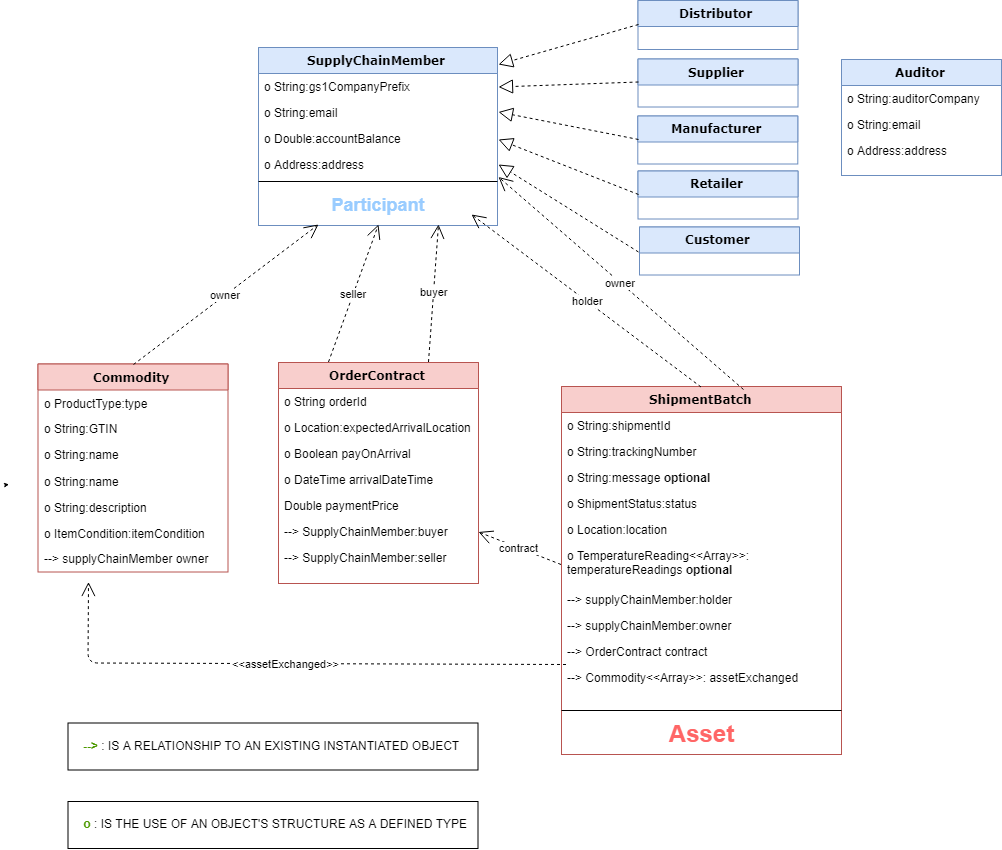
\includegraphics[scale=0.40]{media/participant_asset_relationship.png}
    \caption[Class Diagram for the relationships between assets and participants.]{Class Diagram for the relationships between assets and participants.}
    \label{fig:participant_asset}
\end{figure}

%ASSETS
%CONCEPTS 
%ENUMS

\subsubsection*{Transactions and Transactional Scripts}
The way that the participants an interact with the network and with the assets is through transactions. \textbf{Transactions are the chaincode functions with certain parameters invoked by a user of the network} (how a user can invoke a transaction is another matter, also discussed in the following sections). So, while the participants and assets model the users and data storage of the system, \textbf{the transactions model the behaviour of the network}, by accessing the participant and asset registries and making changes. Any transaction invocation is always recorded in an immutable historical record.

All the creation, deletion and update transactions are already supported by default by Composer, but all other behaviour needs to be modeled, and sometimes, even these default transactions should be made restricted and replaced by custom made ones, to ensure system integrity.


The transactions that were modeled for this network, are featured in the following list, with their descriptions: 
\begin{itemize}
    \item \textbf{CreateShipmentAndContract} - creates a shipment and the associated contract at the same time, for a certain set of parameters, which includes a buyer, seller, the commodities to include in the shipment, etc.
    \item \textbf{UpdateShipment} - update a shipment's tracking status, location and optionally pass it over to a new holder. In case the shipment is being delivered to the buyer, if a payment was established in the contract, it is automatically done. \textbf{Emits a "possible fraud" event when a shipment does not arrive on the expected location, and a normal event warning that the shipment was updated as well}.
    \item \textbf{UpdateCommodity} - A custom transaction to update a commodity, instead of using the default one. The reason is to make access control rules easier for this behaviour easier.
    \item \textbf{DeleteCommodity} - Again, a custom transaction, to delete a commodity. The reason for this transaction being custom is that a verification must be done to check if the commodity is part of a shipment before deleting it. In case it is, to maintain the integrity of the system, the commodity is not deleted
    \item \textbf{ReportDamagedGood} - Sometimes, goods are damaged during their shipment. This transaction updates the current status of a commodity and a description of the occurrence, so that a registry for any damages occurred can be
    \item \textbf{TransformCommodities} - This transaction converts 1 or more commodities in a different set of commodities, by deleting the old ones and creating new ones. It is useful, for instance, when creating a product out of raw materials. \textbf{Emits an event warning that the products were transformed}.
    \item \textbf{TransferCommodityPossession} - transfer the ownership of a commodity to a different participant of the network, but only if the commodity is not currently part of any shipment. \textbf{Emits an event warning about the change of ownership}.
    \item \textbf{TemperatureReading} - Finally, and to ensure full product condition traceability, temperature readings can be inserted into the system. A shipment can log an array of temperature readings, and each time this transaction is called for a shipment, a reading can be inserted into the array.
\end{itemize}

Additionally, the transactions, with all their parameters can be seen in Figure~\ref{fig:full_class_diagram}, from appendix~\ref{chap:appendix-b}.

%\item Tutorial/Show-off the functionalities of some kind? Include this on the 1st point?
\subsubsection*{Queries}
The transactions are used to model actions and behaviour, but to retrieve some of the information, something else is needed. \textbf{Composer already retrieves the basic information for participants, assets and transactions, but anything else requires queries}. Hyperledger Fabric uses a relational database to store the asset and participant registries and Composer features a way to retrieve that data easily, through filtered queries (using a javascript framework, LoopBack).

In this proof of concept, some queries were programmed for some of the most important pieces of information that can ensure traceability and other properties. These can be found in table~\ref{table:queries-list}.

%%%%%%%% TABLE BEGIN %%%%%%%%%%%%%%%

\begin{table}[h]
    \centering
    \caption{List of designed and implemented queries, with their parameters.}
    \label{table:queries-list}
    \begin{tabular}{|l|l|l|l|}
    \hline
    \textbf{ID} & \textbf{Name}                   & \textbf{Retrieve}   & \textbf{Parameters} \\ \hline
    1           & selectShipmentByID              & ShipmentBatch       & Shipment ID         \\ \hline
    2           & selectShipmentByOwner           & ShipmentBatch{[}{]} & Shipment Owner      \\ \hline
    3           & selectShipmentByHolder          & ShipmentBatch{[}{]} & Shipment Holder     \\ \hline
    4           & selectShipmentByCountry         & ShipmentBatch{[}{]} & Location Country    \\ \hline
    5           & selectShipmentByTrackingcode    & ShipmentBatch       & Tracking Number     \\ \hline
    6           & getHistorianRecords             & Transaction{[}{]}   & None                \\ \hline
    7           & getHistorianByPerson            & Transaction{[}{]}   & Participant         \\ \hline
    8           & getHistorianByType              & Transaction{[}{]}   & Transaction Type    \\ \hline
    9           & getDamagedGoodsTransaction      & Transaction{[}{]}   & None                \\ \hline
    10          & getCreatedShipmentsTransactions & Transaction{[}{]}   & None                \\ \hline
    11          & getCommoditiesTransformations   & Transaction{[}{]}   & None                \\ \hline
    12          & getCommodityOwner               & Commodity           & GTIN                \\ \hline
    13          & getShipmentWhereCommodityExists & ShipmentBatch       & Commodity           \\ \hline
    \end{tabular}
    \end{table}

%%%%%%%% TABLE END %%%%%%%%%%%%%%%%%

The queries are pretty straight forward to code. They are a basic SELECT type of query, with the specification of what object we want to select, followed by a WHERE kind of statement, where certain conditions like equality, inequality, \textit{"CONTAINS"} among a few others can be used. 

For instance, query number 12, \textit{getCommodityOwner}, takes as parameter the Commodity's ID (GTIN), but instead of retrieving the owner of the commodity, a participant, it returns the Commodity itself. Why? Because the commodity retrieved has all the information of who the owner is. This information has to be extracted manually since it is \textbf{impossible} to make a query to select only that attribute.

\subsubsection*{Query Difficulties}

Though the ease of coding the queries is appreciated, they are pretty limited in what they can do. For instance, it is impossible to natively nest a \textit{"SELECT"} inside another. Since the database behind is not relational, there are also no powerful query elements like \textit{"JOIN"}, which makes for getting some pieces of information very hard or even impossible. 

To make up for this, some changes in the model had to be made. Originally, the \textit{Commodity} asset did not have a \textit{Owner} data attribute, since it was not thought to be needed. A \textit{ShipmentBatch} has a \textit{Owner}, and a list of \textit{Commodities}. Therefore, if a relational database were used, by providing the ID of a \textit{Commodity} as parameter, it would be possible to retrieve the \textit{Owner}, simply by joining the tables for the shipment, participant and commodity using the given ID, and it would return the owner. In a relational database, any relation points both ways, so it is easy to navigate between the classes of a model, but that does not happen here.



\begin{figure}[h]
    \centering
    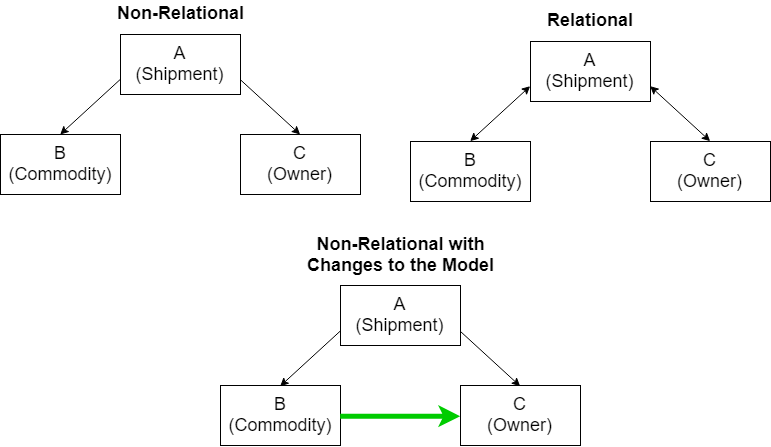
\includegraphics[scale=0.40]{media/relational_problem.png}
    \caption[Exemplification of the non-relational model problem in the Hyperledger Projects.]{Exemplification of the non-relational model problem in the Hyperledger Projects.}
    \label{fig:relational_problem}
\end{figure}
Figure~\ref{fig:relational_problem} illustrates the problem anc changes to the developed model that had to be made to adapt to it. The \textit{Commodity} was adapted to have a \textit{Owner} data attribute so that it is easier to query the owner of a commodity. This pretty simple query would be a lot harder to accomplish in Composer, and anything more complex or having more tables than this would be pretty much impossible to do without exporting all the data to another system that could organize it and query it in a different way. 

Another problem that this can bring, other than having the trouble of changing the model, is the integrity issues that can be caused in the data. Anytime that the owner of a shipment is changed, the owner of the commodity also has to be changed in the code. If the owner of a commodity was not changed in the code, then it would be inconsistent with the owner of the shipment, who in reality should also own the commodity. \textbf{If a programmer consistently adds attributes to classes to make up for the weak Composer queries, eventually they might forget to make a change similar to this one and the system might lose integrity}.


\subsection{Composer Business Network - Identity Management and Access Control}

Creating a model design for the network with all the previously explained items grants the needed basic functionalities for the system to work, but it misses one of the most important aspects from the requirements: \textbf{the security and access control}.

As previously explained in Section~\ref{sec:composer-background}, Composer features the concept of Participant, a network instance of the class that represents a user, but it also features identity cards, which are files that function as the private key and identification card for a real person. An identity card and an instance of a participant can be linked to each other.

The control rules are written to reflect what actions are allowed to certain participant class types, to specific participant instances, and even to specific identity cards. 

%There are 2 ways to \textbf{manage access control in the Composer framework:}
%\begin{itemize}
 %   \item Access Control File - 
  %  \item Programmatic Control in the Transaction Scripts - 
%\end{itemize} focus o
%Identity management - Creating identities, associating them to the participants, etc. (MAYBE THIS IS BETTER OFF IN THE BACKGROUND/STATE OF THE ART SECTION ABOUT COMPOSER)

A set of access control rules was designed with the requirements in mind, so that only certain people can access certain sensible pieces of information, and so that not everyone can manage other people's data. 

 All of these rules were implemented in a mixture of two methods. The first is by using the access control composer language and \textit{.acl} file. The second is to program the transactional scripts to check the identity and data of the person invoking the transaction and then throw errors if the invoker should not have access.

 \textbf{The designed permissions are sectioned by items}, namely the \textbf{transactional data and invocations}, the \textbf{asset data and its CRUD actions} and the \textbf{participant data and its CRUD actions}. The following list features a series of these items, with their name, action and access control rule. The admin identity card is has full access, so it will be mostly omitted from these rules.

\textbf{Permissions and access control rules:}
\par
\par \textbf{Transactions - Invoke}
        \begin{itemize}
		\item CreateShipmentAndContract - Allowed for every participant and identity, excluding the \textbf{customer} participant types;
		\item ReportDamagedGood - Allowed only for the holder of a shipment with the specified commodity;
		\item TemperatureReading - Allowed only for the holder of the shipment with the temperature being read; %-> Prepare the device with the needed business cards)
		\item TransferCommodityPossession - Allowed only for the owner of the commodity.% This commodity can not be part of a shipment at the moment of the transferrence. 
		\item TransformCommodities - Allowed only for the owner of all the commodities that are input arguments. %Therefore, all transformed commodities in a transaction must have the same owner;%, and he may specify a new owner if he so desires % (I can comment 1 single line to make this transaction not change owner)
		\item UpdateShipment - Allowed only for the holder of a shipment;
		\item UpdateCommodity - Allowed only for the owner of a commodity;
		\item DeleteCommodity - Allowed only for the owner of a commodity;
		\end{itemize}
    \par \textbf{Assets}
        \begin{itemize}
        \item Commodity
            \begin{itemize}
			\item Create - Allowed for supply chain member participant type;
			\item Read - Allowed for supply chain member participant type who owns the commodity being read; allowed for the auditor participant type;
			\item Update - Allowed for supply chain member participant type who owns the commodity being Updated;
            \item Delete - Admin only;
            \end{itemize}
        \item OrderContract
            \begin{itemize}
			\item Create, Update, Delete - Admin only;
			\item Read - Allowed for the buyer and seller of the contract; allowed for the auditor participant type;
            \end{itemize}
        \item ShipmentBatch
            \begin{itemize}
			\item Create, Update, Delete - Admin only;
			\item Read - Allowed for the owner and holder of a shipment, as well as the buyer in the shipment's contract; allowed for the auditor participant type;
            \end{itemize}
        \end{itemize}
    \par \textbf{Participants}
        \begin{itemize}
        \item Supply Members
            \begin{itemize}
			\item Create, Update, Delete - Admin only;
            \item Read - Allowed for the auditor participant type; allowed for a participant's own details;
            \end{itemize}
        \item Auditor
            \begin{itemize}
            \item Create, Update, Delete - Admin only;
			\item Read - Auditor can read own details; 
            \end{itemize}
        \end{itemize}

So, these rules reflect some basic facts. Auditors can read anything in the network, while admins can read, update, delete, create or invoke anything. The common users are subject to reading only details from themselves and the assets they are associated to in some way (buyer, owner, holder, etc). In the same way, they are also limited on the transactions they can invoke based on these associations. 

Finally, the CRUD actions that the supply chain members can execute for the assets and participants are also pretty limited, in order to \textbf{maintain system integrity}. This was essential since Composer does not, by default, make some essential integrity checks on the CRUD actions. For instance, when updating an asset's reference to another asset, Composer does not verify if the new reference actually points to an existing instance of an object, which is the reason for why some custom transactions were designed, such as \textit{UpdateCommodity}.

Though all of these access rules were designed, not all were implemented in time, but the ones that were implemented were tested and worked flawlessly.

\subsubsection*{Conclusions and Security Concerns }

In an ending note, identity management is a complex thing in the Composer framework, not only because of the rule design, but also because of how it can be bypassed by \textbf{human error and social engineering}. Nothing, but the immutability of the ledger records, is granted, especially when there is an admin that can control the system.

Additionally, some transaction invocations would be more secure if they could have a multiple signature from many parties. One such transaction could be the \textit{UpdateShipment} transaction. when an item is being delivered to its buyer, it should be made sure that the transaction was acknowledged by both parties, so that the payment could be confirmed securely. \textbf{Such a thing is not yet permitted by this framework and constitutes a grave security fault, therefore not satisfying the security requirements completely}.


\subsection{Network Topology and Deployment}

Composer also features network topology design, which includes choosing the organizations running the network, how many nodes each organization hosts and what types of nodes and the endorsement policy. This is especially useful to quantitatively test the efficiency metrics and scaling of the system, depending on the topological setup. Such measurements are important to compare this system with other possible architectures.

However, the scope of this project covers mostly the qualitative and functional part of building the network, with the aim of finding out if the requirements can successfully be implemented and work as intended, independently of how the network scales and independently of how other architectures behave. Especially in the case of Hyperledger Composer, the implementation so far works, either with just 1 node,nd, even though there was no implementation of a big topological network of nodes, some speculation or with a small number of them. 

With that in mi and thought were given as to how a proper network should look like. Figure~\ref{fig:fabric_topology}, taken from the Fabric documentation, exemplifies how a small supply chain topology would be organized.

\begin{figure}[h]
    \centering
    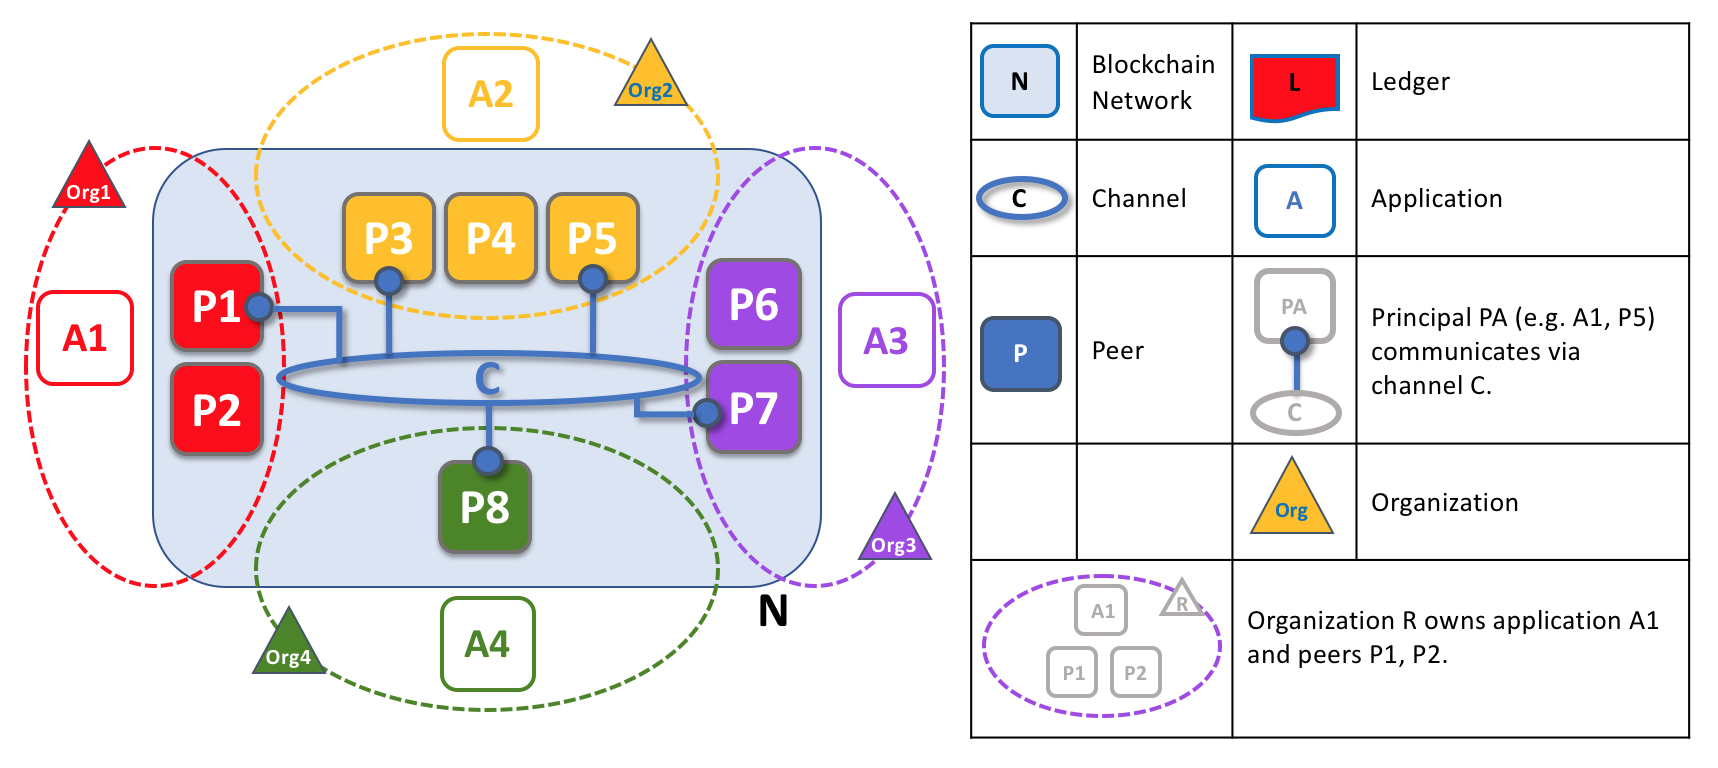
\includegraphics[scale=0.50]{media/fabric_topology.png}
    \caption[Example fabric topology for 3 organizations.]{Example fabric topology for 3 organizations. Adapted from~\cite{FabricDocPeers}}
    \label{fig:fabric_topology}
\end{figure}



%Mention the file for consensus, the file for node topology and for endorsement.
%Deployment diagram explaining how a full network would work.

%Business Network Deployment - Explain how it works in the background through fabric, the nodes, the consensus and the option do define endorsement policy (which was the default as per this design, since no requirements were elicited that required otherwise); Include deployment (physical) diagram and explain the decisions made.

\subsection{Integrating Existing Systems and Building External Applications}

The synchronization requirements were another strong focus points, an issue that deals a lot with building points of access for several external applications to use while importing, exporting data and interacting with the blockchain.

\subsubsection*{Architectural Context Considerations}

An important task of architectural design is identifying where blockchain is in the middle of everything. It was already laid out that it can be used by other applications as the source of truth. \textbf{Architecturally, this may mean that blockchain might be used as the lowest layer} of a network, and that it can even be the support for more than 1 network. 

All the other data layers would get the information from the blockchain, and inject their information to the blockchain, when needed. The upper layers could organize and treat information however they want, as long as they could retrieve it securely. This way, it would even be possible to make up for the shortcomings of the query language of Composer, by retrieving the Blockchain data to a higher level layer application and have that application organize the data in a way that would make it more accessible. Of course, building these upper layers is all up to the developers of each company and application that wants to interact with the blockchain. 

Figure~\ref{fig:architectural_diagram} shows an idealization of what such an architectural layer design would look like. From oracles extracting and inserting big chunks of data periodically, to applications using the blockchain directly as their data storage source, the possibilities for the layers above the blockchain network are many, and not even limited to what can be seen in the figure.

\begin{figure}[h]
    \centering
    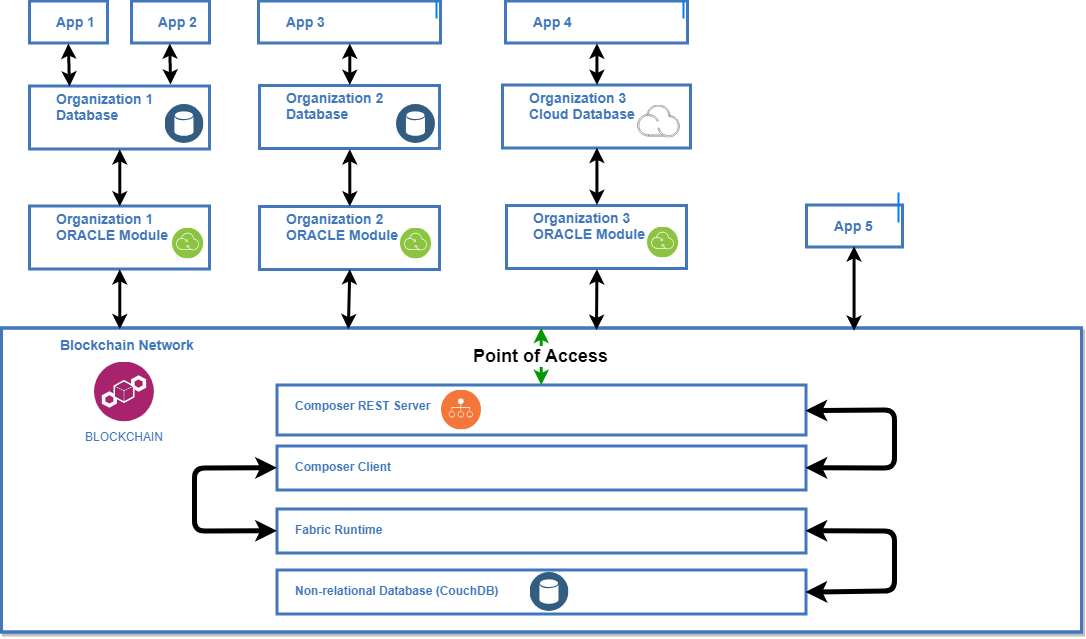
\includegraphics[scale=0.40]{media/architectural_diagram.png}
    \caption[Architectural layer representation of Blockchain Integration with other systems.]{Architectural layer representation of Blockchain Integration with other systems.}
    \label{fig:architectural_diagram}
\end{figure}

\textbf{The integration part of this project deals with defining secure and authenticated points of access for the upper layers to have access to.}

\subsubsection*{REST Server API and Authentication}
Composer already features a ready-to-start API server, which includes all the transaction invocations, queries and CRUD operations. Authentication, using identity card files, is also included in the REST server's functionalities.

It is also possible to write a custom REST server for composer, using Angular applications, but the default server has the necessary features.

\subsubsection*{Other Applications}
Other software are possible to be implemented with the blockchain. One such instance of a software is Node-RED, to connect the blockchain to an IoT network of devices, especially important in case we want to achieve traceability of product conditions or quickly scan products. It can also be used to subscribe to network events.